\section{Model selection}

\subsection{Multicollinearity on full model}

Before doing any model selection, we first check if we have any multicollinearity problem. We saw in the last part that some variables were highly correlated. These high pairwise correlations could lead to multicollinearity problem but it is not always the case.

Let the full model be, 
\begin{equation}
	Y = X\beta + \varepsilon
\end{equation}

To verify that, we can use the \textbf{Variance inflation factor (VIF)} that is defined by for the coefficient $\hat{\beta}_k$,

\begin{equation}
	\text{VIF}_k = \frac{1}{1 - R^2_k}, \quad k = 1,...p-1
\end{equation}

where $R^2_k$ is the coefficient of determination of a regression of $X_k$ on $X_1,\dots,X_{k-1},X_{k+1},\dots,X_{p-1}$. Multicollinearity leads to an "ill-conditionned" matrix $X$. As a consequence, this matrix is numerically instable and becomes difficult to invert. Therefore, the OLS estimator $\hat{\beta}$ cannot be "correctly" computed.
We have multicollinearity problem if the \textbf{VIF} is greater than $10$ and if the \textbf{average VIF} is much greater than $1$. We can also check the tolerance which is $1 - R^2_k$.

In the appendix (\ref{fig:vif_full_model}), you can find a table with the VIF and tolerance for each variable of the full model. We notice a multicollinearity problem for the variables \textit{gpd} (with VIF $= 13.10$) and \textit{income.composition.of.resources} (with VIF $= 12.72$). These two have tolerance of $0.08$. Furthermore, the average VIF is $4.67$. %Therefore we can already remove these two variables from our model.

In order to fix this multicollinearity problem, we can perform a \textbf{Ridge regression} that is similar to the OLS in the sense it minimizes the SSR but it also adds a constraint on the $L_2$ norm (euclidean) for $\beta$. The constraint is,
\begin{equation}
	||\beta||^2_2 \leq t
\end{equation}
where $t \in \R$ is a parameter to be determined.


To improve our model accuracy, we need to carefully select variables without adding too much to avoid overfitting. To do that, we will perform model selection using \textit{AIC}, \textit{BIC} and \textit{$R^2_a$} criterions. Since we have a lots a variables in our full model, we will only consider model selection of type II and III.

\subsection{Type II: Backward stepwise selection}

The goal of a backward stepwise selection is to start from the full model then gradually removing variables one at a time. At each iteration, we remove the one that yields the lowest accuracy in prediction when added the pool of selected variables. We can measure the accuracy using different criterions, for this project, we will focus on \textit{AIC} and \textit{BIC} criterions.

\subsubsection{Akaike Information Criterion (AIC)}

We want to minimize the AIC that is,
\begin{equation}
	\text{AIC} = - 2 \ln L(\hat{\beta}) + 2k
\end{equation} 
where $L(\hat{\beta})$ is the maximum of the likelihood function and $p$ is the number of estimated parameters in the model.

\subsubsection{Bayes Information Criterion (BIC)}

The problem with AIC is that it tends to select too much variables and therefore overfit the model. We can then use another criterions that penalyzes more severely complex models and tends to favorize simpler models. This criterion we want to minize is the BIC and is given by, 
\begin{equation}
	\text{BIC} = - 2 \ln L(\hat{\beta}) + (2k \cdot \ln(n))
\end{equation}
where $n$ is the number of observations in our training dataset.

\subsection{Type III: LASSO}

The LASSO estimator is similar to the OLS (it minimizes the SSR) but it adds a constraint on the $L_1$ norm (Manhattan) for $\beta$. The constaints is,
\begin{equation}
	\sum_{j=1}^{p} |\beta_j| \leq t
\end{equation}
where $t \in \R$ is a parameter to be determined.

This change allows some coefficients to be shrunk exactly to zero.

\subsection{Interactions between variables}

We should then try to add interactions betweem variables to our chosen model. We decide to test the following interactions and compare the resulting models with our chosen one,

\begin{itemize}
	\item \textit{infant.deaths} with \textit{measles}
	\item \textit{adult.mortality.high} with \textit{alcohol}
	\item \textit{adult.mortality.very\_high} with \textit{alcohol}
	\item \textit{total.expanditure} with \textit{adult.mortality.low}
	\item \textit{total.expanditure} with \textit{infant.deaths}
\end{itemize}

\subsection{Verifying underlying hypotheses}

After selecting a model, we want to check the underlying hypothesis of the linear model. We will verify the 3 main hypothesis: homoskedasticity, independance of observations and normality of the residuals. we will also check for outliers, autocorrelation and nonlinearity.

\subsubsection{Nonlinearity}

We can check for nonlinearity by looking at the scatterplot of the residuals ($e_i$) versus the explanatory variables.

\begin{figure}[H]
	\centering
	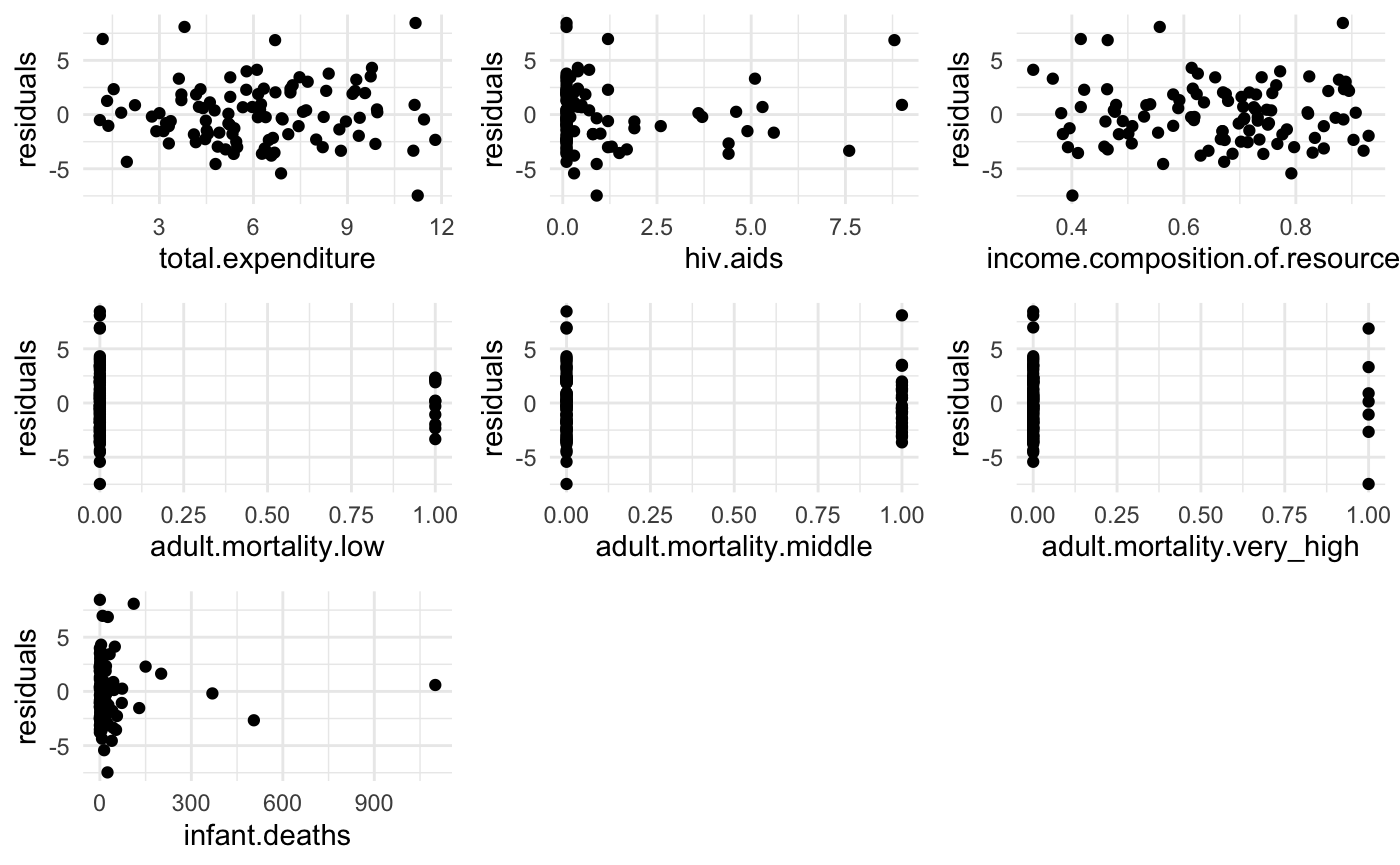
\includegraphics{figures/residuals_vs_explanatory.png}
	\caption{scatterplots of residuals versus explanatory variables for the selected model}
	\label{fig:residuals_vs_explanatory}
\end{figure}

We do not see clear nonlinear patterns in the different plots above. Every variable has more or less a linear relation with its residuals. The continuous variables \textit{hiv.aids} and \textit{infant.deaths} have a strange pattern but the nonlinear seems too complicated to infer and would add a lot of complexity to our model. Therefore, we do not take remedial actions.

\subsubsection{Outliers and influential observations}

a) outliers with respect to the explanatory variables

We first try to identify outliers with respect to the explanatory variables $X_{ij}$. 

We need to study the leverages that are the diagonal elements of the hat matrix $H = X(X^T X)^{-1}X^T$. We can say that $X_i$ is an outlier if,
\begin{equation*}
	h_{ii} > \frac{2p}{n} \approx 0.155
\end{equation*}

We find $12$ outliers that are the following rows of our dataset: $9$, $11$, $12$, $23$, $35$, $40$, $42$, $49$, $58$, $65$, $82$, $97$.

We want then know if the outliers found are influentials for the their fitted values. We use the DFFITS criterion for the i-th observation,
\begin{equation}
	\text{DFFITS}_i = d_i^{\ast} \sqrt{\frac{h_{ii}}{1 - h_{ii}}}
\end{equation}
where $d_i^{\ast}$ are the standardized deleted residuals,
\begin{equation}
	d_i^{\ast} = e_i \sqrt{\frac{n - p - 1}{\text{SSE}(1 - h_{ii}) - e_i^2}} 
\end{equation}

We have a criterion for DFFITS. For $n > 30$, the i-th observation is influential for its fitted value if, 
\begin{equation}
	|\text{DFFITS}_i| > 2 \sqrt{\frac{p}{n}} \approx 0.557
\end{equation}

We find that $8$ observations are influentials for the fitted values: $2$, $9$, $35$, $42$, $49$, $58$, $95$, $96$. Therefore, the observations $9$, $35$, $42$, $49$ are outliers and influentials for the fitted values.

\begin{figure}[H]
	\centering
	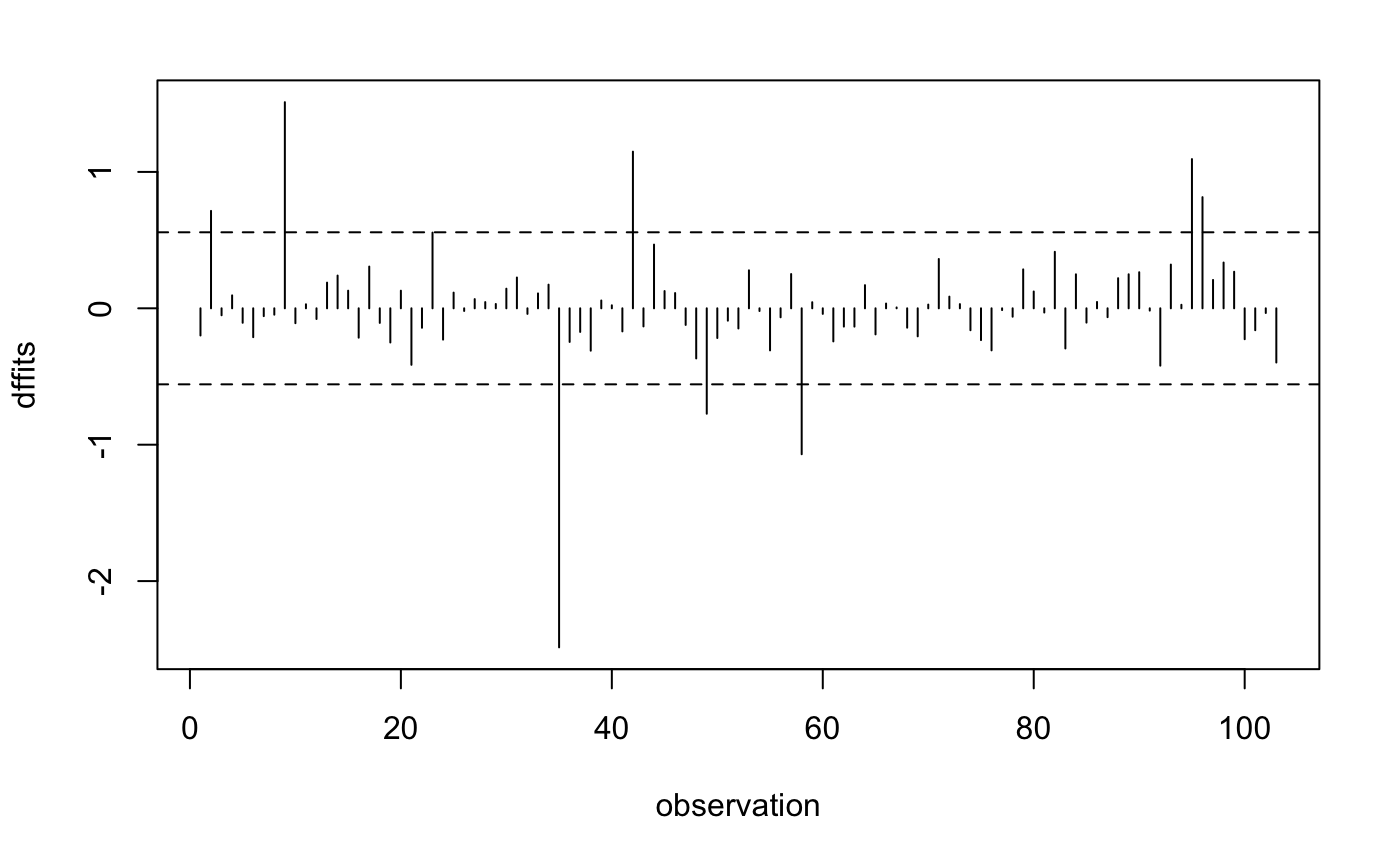
\includegraphics{figures/outliers_influentials_fitted_values.png}
	\caption{outside the two lines are outliers influentials for their fitted values}
	\label{fig}
\end{figure}

Now, are they also influentials for the regression coefficients ? Let's have a look at the Cook's distance.

\begin{figure}[H]
	\centering
	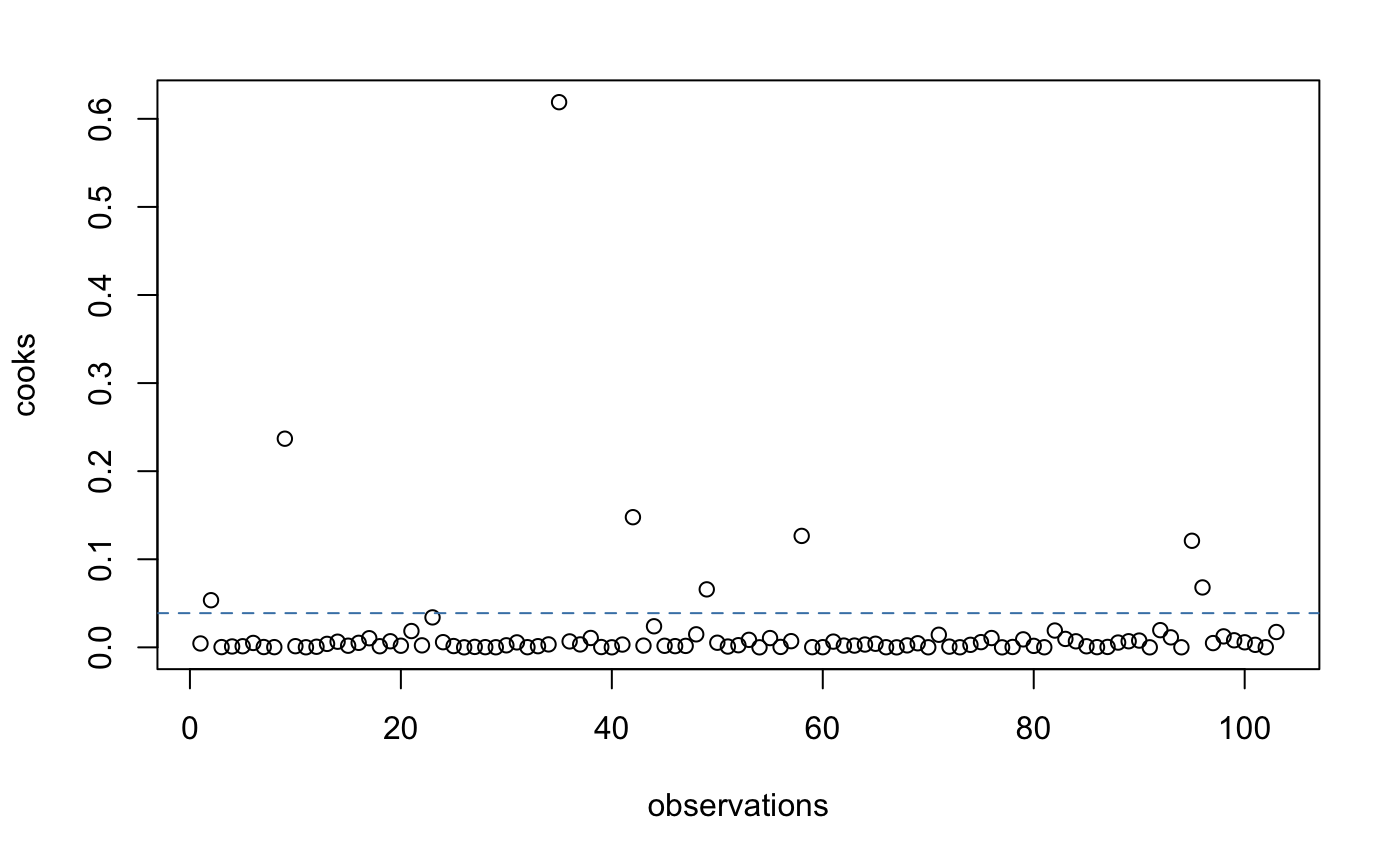
\includegraphics{figures/cooks_distance.png}
	\caption{Cook's distance}
	\label{fig}
\end{figure}

We find that the same $8$ observations influentials for the fitted values are also influentials for the 

% We also want to know if the outliers are influentials for the regression coefficients. We use the DFBETAS criterion for the i-th observation and k-th coefficient $\hat{\beta}_k$, 
% \begin{equation}
% 	|\text{DFBETAS}_{k,i}| > \frac{2}{\sqrt{n}}
% \end{equation}
% where 
% \begin{equation}
% 	\text{DFBETAS}_{k,i} = \frac{\hat{\beta}_k}{\hat{\beta}_{k,i}}{\text{MSE}_i \cdot c_k}, \quad c_k = (X^T X)^{-1}_{kk}
% \end{equation}

% TODO: compute + plot of the DFBETAS vs observations

% We can have an overview of the influentials by looking at the Cook's distance given by, 
% \begin{align}
% 	D_i 
% 		&= \frac{(\hat{\beta} - \hat{\beta}_{i})^T \cdot (X^T X) \cdot (\hat{\beta} - \hat{\beta}_{i})}{p \cdot \text{MSE}} \\
% 		&= \frac{(\hat{T} - \hat{Y}_{i})^T \cdot (\hat{\Y} - \hat{\Y}_{i})}{p \cdot \text{MSE}}
% \end{align}

The i-th observation is influentials if $D_i > F_{p,n-p;1-\alpha}$ where $D_i$ is the Cook's distance

% TODO: compute + plot of cook's distance vs observations

b) outliers with respect to the response variable

We then identify outliers with respect to the response variable $Y_i$. $Y_i$ is an outliers if $d_i^{\ast} > t_{n-p-1;1 - \frac{\alpha}{2}}$. For a level of significance of $\alpha = 0.05$, we have $t_{94 ; 0.975}$ and we find that the observations $2$, $9$, $95$ and $96$ are outliers for the response variable.

\subsubsection{Multicollinearity}

\begin{figure}[H]
	\centering
	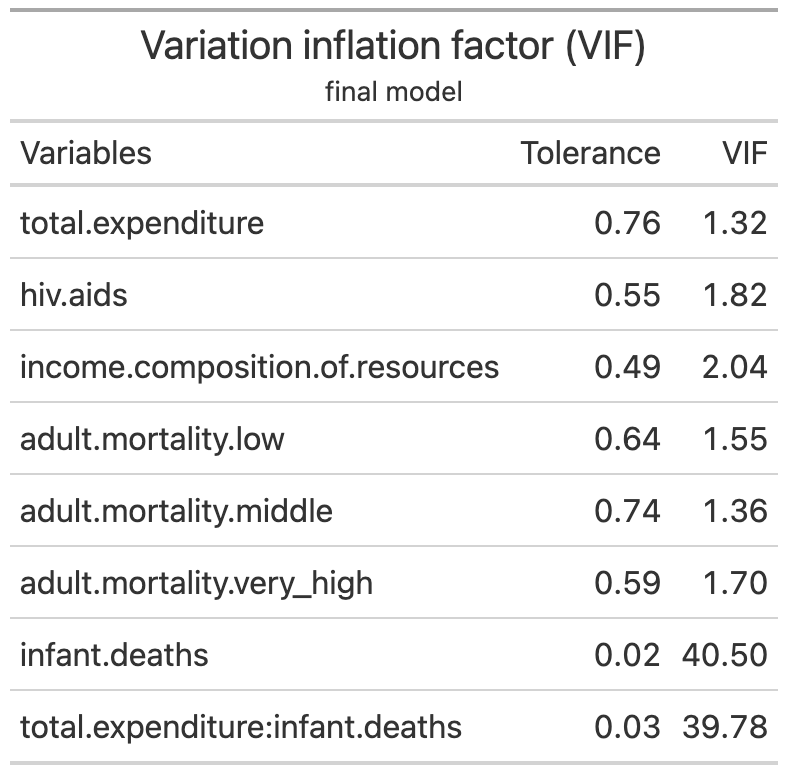
\includegraphics{figures/vif_final_model.png}
	\caption{VIF for the selected model}
	\label{<label>}
\end{figure}

\subsubsection{Heteroskedasticity}

We can check for heteroskedasticity by looking at the plot of the residuals versus the fitted values.

% TODO: plot of residuals vs fitted values + interpretation

\begin{figure}[H]
	\centering
	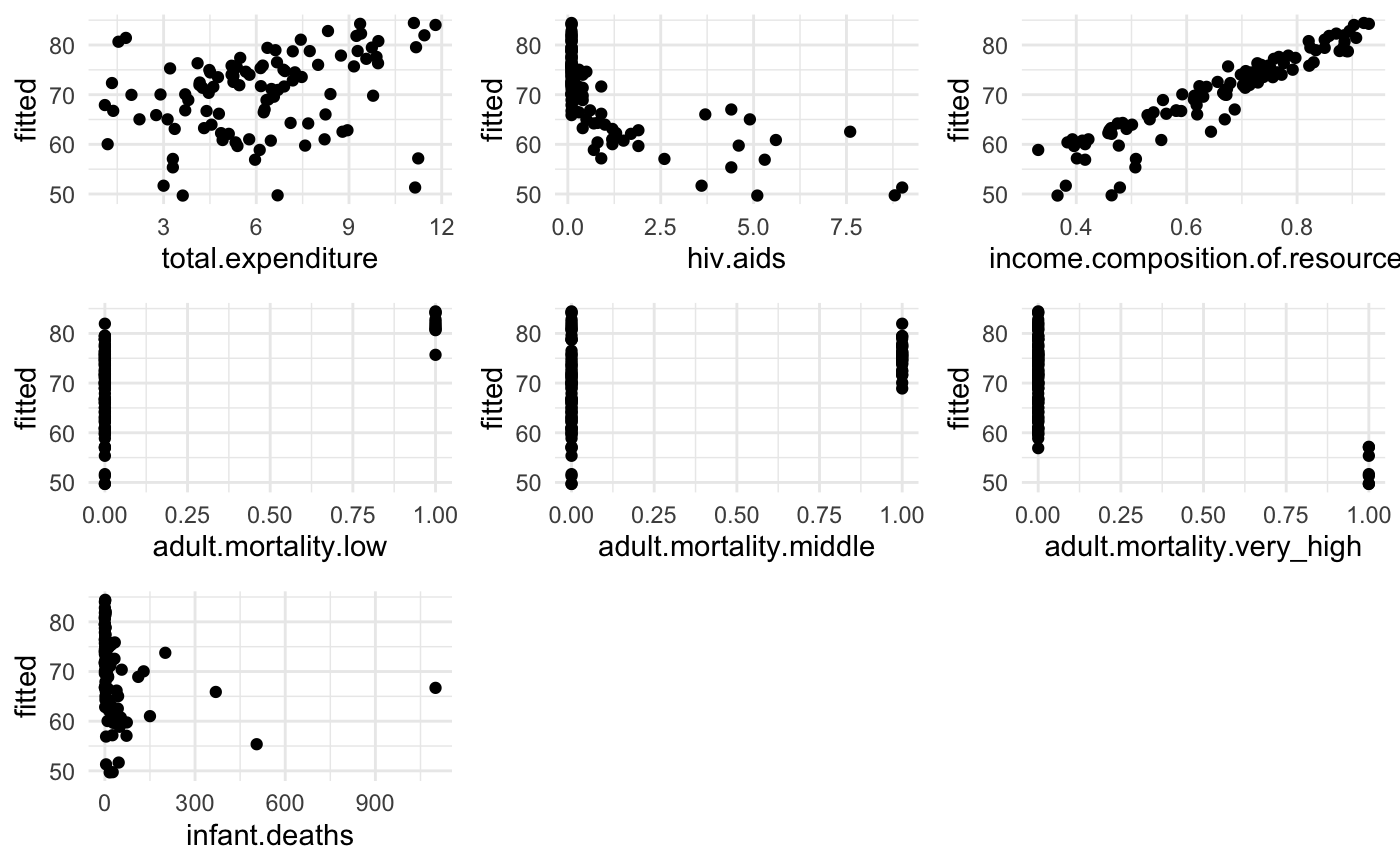
\includegraphics{figures/residuals_vs_fitted.png}
	\caption{scatterplots of residuals versus fitted values for the selected model}
	\label{fig:residuals_vs_fitted}
\end{figure}

However, the best way to determinate if there is heteroskedasticity is to perform the \textbf{White test}. The hypothesis are,
\begin{align*}
	H_0&: \text{there is homoscedasticity} \\
	H_1&: \text{there is heteroskedasticity}
\end{align*}

% TODO: show output of the White test

The p-value of the \textbf{White test} is $0.01729$. At a significance level of $\alpha = 0.05$, we reject the null hypothesis and therefore we can conclude there is \textbf{heteroskedasticity}.

% TODO: taking remedial actions

\subsubsection{Autocorrelation}

We can check for autocorrelation by performing the \textbf{Breusch-Godfrey test}. The hypotheses are,
\begin{align*}
	H_0&: \text{there is no autocorrelation} \\
	H_1&: \text{there is autocorrelation}
\end{align*}

% TODO: show output of the Breusch-Godfrey test

The p-value of the \textbf{Breusch-Godfrey test} is $0.938$. At a significance level of $\alpha = 0.05$, we fail to reject the null hypothesis and therefore we can conclude there is \textbf{no autocorrelation}. 

\subsection{Normality of the residuals}

Considering the Normal Q-Q plot of the residuals comparing the quantiles of the residuals versus the quantiles of a normal distribution. If the residuals are normal, the points on the following plot should follow the straight line,

% TODO: plot of Normal QQplot

Looking at this plot, we see that globally the points follow the straight line so the residuals are normals.  

To ensure there is no a problem ofnormality for the residuals, we can perform a \textbf{Jarque Bera test}. 

Let $S$ be the skewness and $\kappa$ of the residuals. The \textbf{Jarque Bera test} is given by, 
\begin{equation}
	\text{JB} = \frac{n}{6} \left(S^2 + \frac{(\kappa - 3)^2}{4} \right)
\end{equation}

The hypothesis are, 
\begin{align*}
	H_0&: \text{JB} \sim X^2_2 \\
	H_1&: \text{residuals are not normally distributed}
\end{align*}

% TODO: show output of the Jarque-Bera test
\begin{figure}[H]
	\centering
	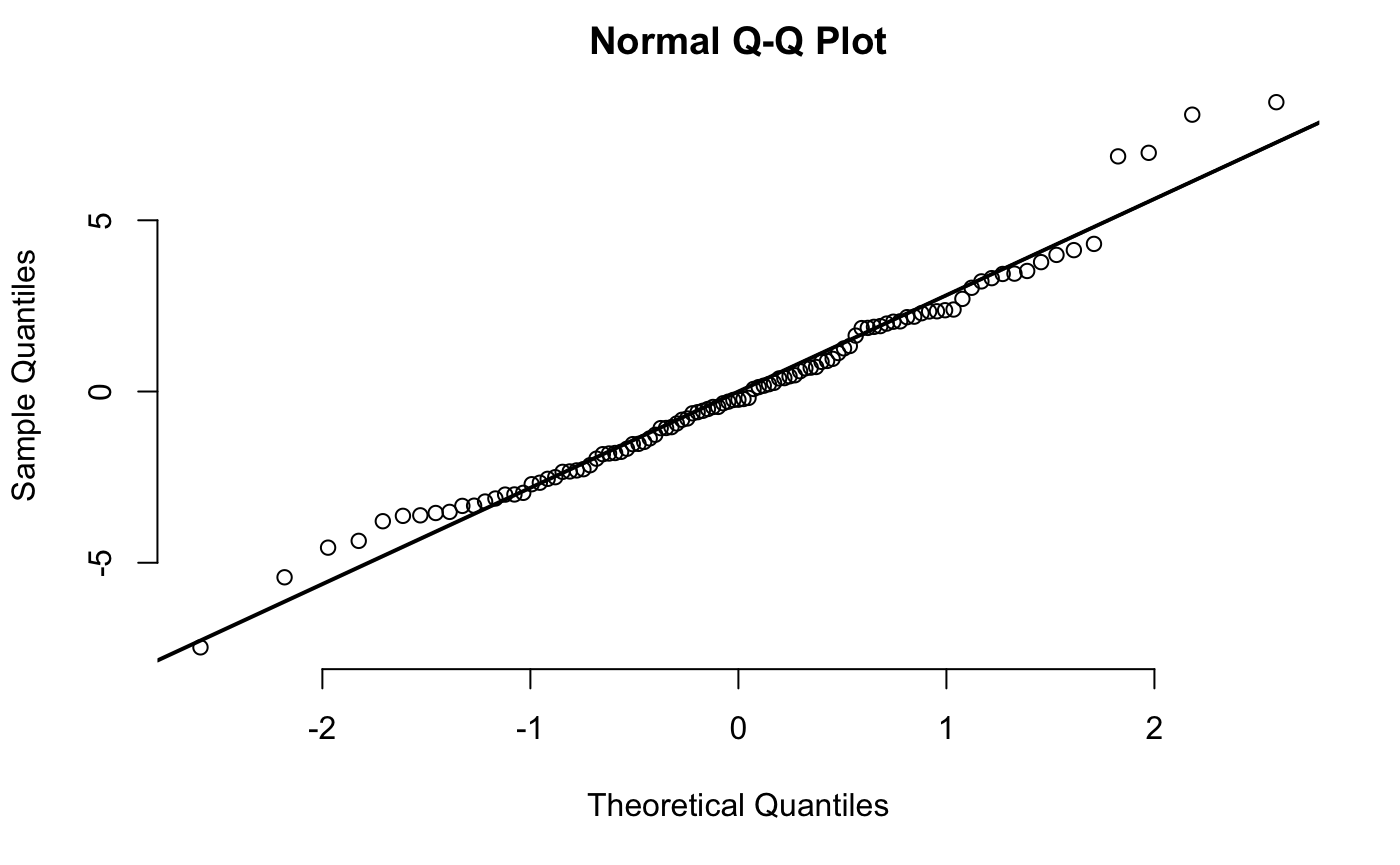
\includegraphics{figures/normal-qq-plot.png}
	\caption{Normal QQ plot}
	\label{fig}
\end{figure}

The p-value of the \textbf{Jarque Bera test} is $0.9287$. At a significance level of $\alpha = 0.05$, we fail to reject the null hypothesis and therefore we can conclude the \textbf{residuals are normaly distributed}. 